% !TeX spellcheck = ru_RU
% !TEX root = vkr.tex

\section{Требования к сервису}
 Проанализировав сущестующие решения, выявлены следующие требования к сервису:
 \begin{itemize}
      \item Удобство поиска товаров и услуг.
      \item Современный и интуитивно понятный интерфейс.
      \item Наличие способов комуникации.
\end{itemize}

От системы отзывов и рейтингов было решено отказаться в виду специфики платформы, так как она
в первую очередь предназначена для волонтеров и небезразличных к судьбе животным людей.

\section{Внешний вид}
Перед тем как непосредственно реализовывать раздел, была продумана его структура. Работа началась с наброска необходимых компонентов и их взаимодействия.
Раздел был разделен на
\begin{itemize}
      \item Основной компонент, представляющий весь раздел.
      \item Компонент поля фильтров.
      \item Компонент карточки отловщика, которая в свою очередь содержит в себе следующие компоненты:
      \begin{itemize}
            \item Компонент, отвечающий за стоимость отловщика.
            \item Компонент, отвечающий за кнопку "добавить в избранное".
      \end{itemize}
\end{itemize}

Следующим шагом было реализовать перечисленные компоненты, используя html и ccss, а также добавить динамическое обновление шаблона, в зависимости от данные отловщика.
Подгрузка данных отловщика была сделана за счет интерполяции~\cite{interpolation}, реализованной в angular и ngClass~\cite{ngClass}, директивы angular,
позволяющей добавлять CSS-классы к элементу в зависимости от данных отловщика. В случае когда элемент мог иметь больше 2х представлений, например цена отловщика, были
использованы такие инструменты как pipe~\cite{pipes}, позволяющие в зависимости от входных данных выдать необходимый ответ.
в html шаблоне к параметру исходной ссылки изображения применяется pipe trapperType.
Код компонентов доступен в репозитории GitHub~\cite{github}.

\begin{listing}
      \caption{Код pipe trapperType}
      \begin{minted}[frame=single]{typescript}

<img class="trapper_type"  [src] = "trapper.animalChoice |
                                    trapperType" >

@Pipe({
  name: 'trapperType',
  standalone: true
})
export class TrapperTypePipe implements PipeTransform {

  transform(value: string): string {
    if (value == "cats") return "../assets/icons/cat.png"
    else if (value == "dogs") return "../assets/icons/dog.png"
    else return "../assets/icons/cadog.png"
  }

}
    \end{minted}
  \end{listing}





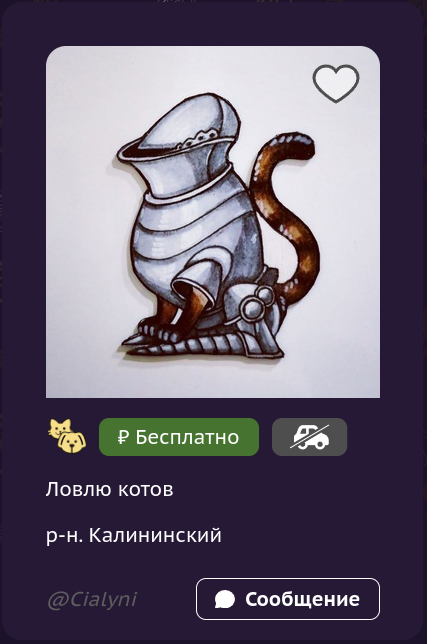
\includegraphics{figures/trappers/card_trapper.png}
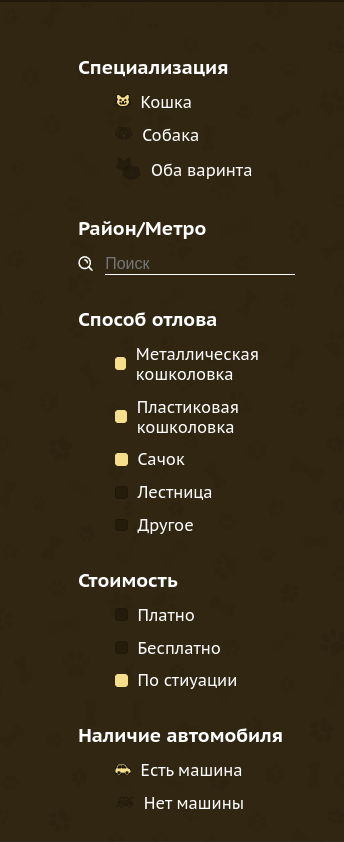
\includegraphics{figures/trappers/filtr-bar.png}



\section{Взаимодействие клиентской части с серверной}

Для корректной работы разделу необходимо:
\begin{itemize}
      \item Получать профили отловщиков с сервера.
      \item Филтровать профили исходя из заданных фильтров.
      \item Обновлять данные на html шаблонах
\end{itemize}

Для обращения к серверу был создан сервис~\cite{services} TrapperProfileService реализующий отправку HTTP-GET~\cite{http-get} запроса с списком переменных, отвечающих за фильтрацию
\begin{listing}
      \caption{Код сервиса TrapperProfileService}
      \begin{minted}[frame=single]{typescript}
@Injectable({
  providedIn: 'root'
})
export class TrapperProfileService {

  private apiUrl = environment.apiUrl;

  constructor(private http: HttpClient) { }

  getTrappersProfile(filterTags: boolean[]) {
    const params = new HttpParams()
    if (filterTags.length != 0){
      const params = new HttpParams()
          .set("isCat", filterTags[0].toString())
          .set("isDog", filterTags[1].toString())
          .set("isCadog", filterTags[2].toString())
          .set("isFree", filterTags[3].toString())
          .set("isPay", filterTags[4].toString())
          .set("isDeal", filterTags[5].toString())
          .set("isMetallCatNap", filterTags[6].toString())
          .set("isPlasticCatNap", filterTags[7].toString())
          .set("isNet", filterTags[8].toString())
          .set("isLadder", filterTags[9].toString())
          .set("isOther", filterTags[10].toString())
          .set("haveCar", filterTags[11].toString())
          .set("haventCar", filterTags[12].toString())
      }
    return this.http.get<Trapper[]>(`${this.apiUrl}/trappers`,
     {params})
  }
}
    \end{minted}
  \end{listing}

Для хранения профилей отловщиков и их обновления в зависимости от фильтров был создан сервис TrapperService.
Также сервис обеспечивает доступ к данным отловщиков для их обновления компонентам.
сервис реализует в себе метод updateTrappersData, принимающий в качестве аргумента массив булеан, отвечающий за фильтрацию, который обновляет атрибут, хранящий данные отловщиков.
Обновления данных происходит за счет сервиса TrapperProfileService


\begin{listing}
      \caption{Код сервиса TrapperService}
      \begin{minted}[frame=single]{typescript}
@Injectable({
  providedIn: 'root'
})
export class TrapperService {
  trapperProfileService = inject(TrapperProfileService)
  trappers: Trapper[] = []
  constructor() {this.updateTrappersData([])}
  updateTrappersData(filter: boolean[]){
    this.trapperProfileService.getTrappersProfile(filter)
    .subscribe(val => {
      this.trappers = val
    })
  }
}
    \end{minted}
\end{listing}
